\chapter{Analyse sur échantillons mixtes}
\label{sec:analyse_mixte}

\section{Motivation et cadre réaliste}
\label{sec:motivation_mixte}

Les chapitres précédents ont permis d’étudier séparément deux problématiques complémentaires : l’identification des particules hadroniques dans le SDHCAL, puis la reconstruction de leur énergie incidente. Dans ces études préliminaires, chaque espèce de particule était traitée indépendamment, ce qui revient à supposer connue a priori la nature de la particule entrant dans le calorimètre.

Une telle hypothèse constitue un cadre idéalisé, utile pour caractériser les performances intrinsèques des méthodes développées, mais elle reste insuffisante dans la perspective d’une utilisation expérimentale réaliste. En pratique, un détecteur reçoit simultanément différentes espèces de particules, et l’information disponible en amont ne permet pas toujours de distinguer immédiatement un pion, un proton ou un hadron neutre. La reconstruction de l’énergie doit alors être effectuée dans un contexte où l’identité de la particule n’est pas connue avec certitude.

Cette situation introduit un couplage direct entre les deux tâches étudiées précédemment :

\begin{itemize}
    \item \textbf{identifier} la particule incidente à partir de la topologie de sa gerbe ;
    \item \textbf{reconstruire} son énergie en appliquant la calibration la plus adaptée.
\end{itemize}

Autrement dit, la qualité de la reconstruction énergétique dépend désormais de la qualité du classificateur PID. Une erreur d’identification peut conduire à appliquer un estimateur optimisé pour une autre espèce, et donc introduire un biais systématique sur l’énergie reconstruite.

Cet enjeu est particulièrement important dans les approches modernes de type \emph{Particle Flow Algorithm} (PFA), où la reconstruction globale d’un événement repose sur la combinaison cohérente de plusieurs sous-détecteurs. Dans ce cadre, une bonne identification hadronique améliore non seulement la pureté des objets reconstruits, mais aussi la précision de la mesure énergétique associée.

L’objectif de ce chapitre est donc d’évaluer les performances d’une chaîne complète de reconstruction dans un environnement mixte, plus proche des conditions expérimentales réelles. Trois stratégies sont comparées :

\begin{itemize}
    \item une chaîne \textbf{PID + régression LightGBM}, où l’espèce prédite détermine le modèle d’énergie utilisé ;
    
    \item une chaîne \textbf{PID + méthode paramétrique}, fondée sur les calibrations analytiques spécifiques à chaque espèce ;
    
    \item une approche de référence consistant à appliquer une \textbf{calibration unique issue des pions} à toutes les particules, sans identification préalable.
\end{itemize}

La comparaison de ces scénarios permet de quantifier l’apport réel du PID sur la reconstruction calorimétrique, d’identifier les limitations dues aux confusions entre espèces, et d’évaluer quelles stratégies apparaissent les plus robustes pour une application future sur données réalistes.

%%%%%%%%%%%%%%%%%%%%%%%%%%%%%%%%%%%%%%%%%%%%%%%%%%%
\section{Chaîne complète : PID + régression BDT}
\label{subsec:mix_pid_bdt}

La première stratégie étudiée consiste à combiner le classificateur de particules présenté au chapitre précédent avec les modèles de régression LightGBM dédiés à la reconstruction d’énergie. Pour chaque événement du faisceau mixte, une étape d’identification est d’abord réalisée entre les classes pion \(\pi^-\) et proton \(p\). L’énergie est ensuite estimée à l’aide du modèle de régression correspondant à l’espèce prédite.

Cette approche reproduit un scénario réaliste dans lequel plusieurs calibrations spécialisées sont disponibles, mais où leur sélection dépend directement de la performance du PID.

\subsection*{Linéarité de la réponse}

La Figure~\ref{fig:linearite_pid_bdt_new} présente la moyenne de l’énergie reconstruite en fonction de l’énergie vraie, ainsi que le biais relatif défini par :

\[
\delta(E)=
\frac{\langle E_{\mathrm{reco}}\rangle-E_{\mathrm{true}}}{E_{\mathrm{true}}}.
\]

Globalement, la réponse reconstruite reste très proche de la diagonale idéale sur l’ensemble du domaine étudié. Les deux espèces suivent une évolution régulière, sans rupture visible, ce qui confirme la stabilité de la chaîne complète PID + régression.

À basse énergie, un léger biais positif est observé. Il atteint environ \(+10\,\%\) pour les pions autour de \SI{10}{GeV}, tandis qu’il reste plus modéré pour les protons (\(\sim +3\) à \(+4\,\%\)). Cette surestimation diminue progressivement avec l’énergie.

Entre \SIrange{40}{80}{GeV}, le biais devient faible pour les deux classes, généralement contenu dans une bande de quelques pourcents autour de zéro. Cette région correspond au domaine où les performances globales du modèle sont les meilleures.

À plus haute énergie, une légère sous-réponse apparaît. À \SI{100}{GeV}, elle reste toutefois modérée, de l’ordre de \(-1\) à \(-2\,\%\), ce qui traduit une excellente linéarité globale.

\begin{figure}[!ht]
\centering
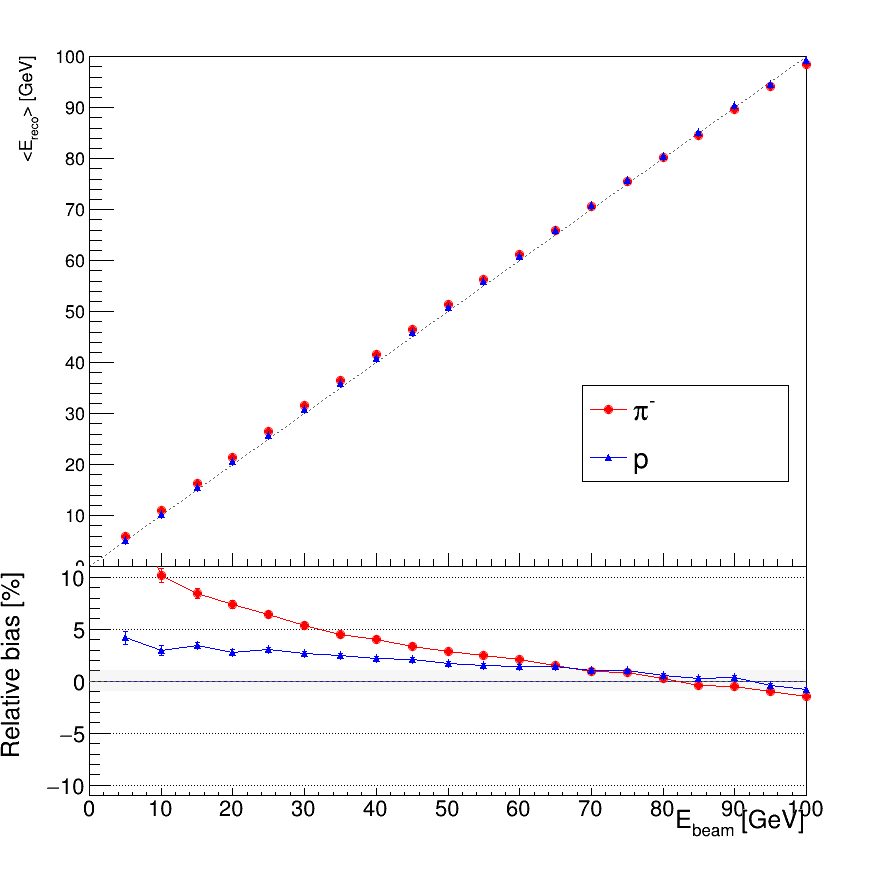
\includegraphics[width=0.78\linewidth]{Fig/PID_Lin_n_Dev_BDT.png}
\caption{Linéarité de la reconstruction d’énergie et biais relatif pour la chaîne complète \textbf{PID + BDT}. Les pions sont représentés en rouge et les protons en bleu.}
\label{fig:linearite_pid_bdt_new}
\end{figure}

\subsection*{Résolution énergétique}

La Figure~\ref{fig:resolution_pid_bdt_new} montre l’évolution de la résolution relative :

\[
\frac{\sigma_E}{E},
\]

extraite à partir d’un ajustement gaussien des distributions résiduelles dans chaque bin d’énergie.

Comme attendu pour un calorimètre hadronique, la résolution décroît rapidement lorsque l’énergie augmente. Elle passe d’environ \(19\,\%\) à basse énergie à des valeurs proches de \(8\,\%\) autour de \SI{100}{GeV}.

Les protons présentent systématiquement une résolution légèrement meilleure que celle des pions, avec un avantage typique de quelques dixièmes à un point de pourcentage selon l’énergie. Cette hiérarchie est cohérente avec les observations faites dans le cas idéal, où les gerbes protoniques apparaissaient légèrement plus stables.

À haute énergie, les deux courbes convergent vers des performances très proches, signe que l’impact des erreurs de PID devient secondaire lorsque la statistique de gerbe augmente.

\begin{figure}[!ht]
\centering
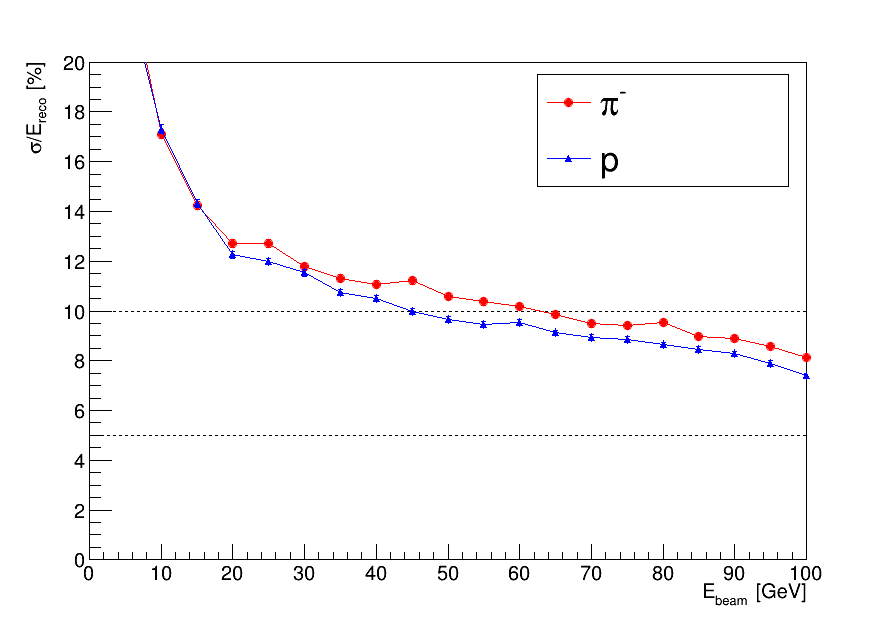
\includegraphics[width=0.78\linewidth]{Fig/PID_Resolution_relative_BDT.png}
\caption{Résolution relative \(\sigma(E)/E\) obtenue avec la chaîne \textbf{PID + BDT}.}
\label{fig:resolution_pid_bdt_new}
\end{figure}

\subsection*{Interprétation physique}

Ces résultats montrent que la combinaison d’un PID supervisé avec une régression dédiée par espèce permet de conserver l’essentiel des performances obtenues dans le scénario idéal où la particule est supposée connue.

Le biais positif observé à basse énergie peut s’expliquer par la faible multiplicité de hits et par les fluctuations importantes des premières interactions hadroniques, qui rendent simultanément l’identification et la régression plus délicates.

La légère supériorité des protons en résolution suggère que leurs gerbes sont, dans cette configuration, un peu mieux modélisées par les variables d’entrée utilisées pour la régression.

Enfin, la faiblesse des biais résiduels à moyenne et haute énergie indique que les erreurs de classification pion/proton n’induisent qu’une dégradation limitée sur la reconstruction finale.

\subsection*{Bilan}

Parmi les stratégies étudiées, la chaîne \textbf{PID + BDT} apparaît comme la plus performante et la plus robuste. Elle combine une excellente linéarité, une résolution compétitive sur tout le domaine énergétique, et une faible sensibilité aux confusions résiduelles du classificateur. Elle constitue ainsi une référence solide pour une reconstruction hadronique réaliste dans le SDHCAL.
%%%%%%%%%%%%%%%%%%%%%%%%%%%%%%%%%%%%%%%%%%%%%%%%%%%%%

\section{Chaîne complète : PID + reconstruction paramétrique}
\label{subsec:mix_pid_param}

La seconde stratégie consiste à conserver la même étape d’identification des particules, mais à remplacer la régression par arbres boostés par la méthode analytique fondée sur les compteurs semi-digitaux aux trois seuils. Une fois la particule classée comme pion \(\pi^-\) ou proton \(p\), les coefficients de calibration spécifiques à cette espèce sont appliqués afin d’estimer l’énergie incidente.

Cette approche est plus simple et plus interprétable que la régression BDT. Elle permet également d’évaluer dans quelle mesure une calibration paramétrique classique reste compétitive lorsqu’elle est couplée à une étape de PID.

\subsection*{Linéarité de la réponse}

La Figure~\ref{fig:linearite_pid_param_new} présente la réponse moyenne reconstruite ainsi que le biais relatif en fonction de l’énergie vraie.

La tendance générale reste linéaire sur l’ensemble du domaine étudié, mais un biais négatif apparaît progressivement lorsque l’énergie augmente. Après une zone relativement bien calibrée entre \SIrange{20}{50}{GeV}, les deux espèces présentent une sous-réponse croissante.

À \SI{100}{GeV}, le biais atteint environ \(-9\,\%\) pour les pions et \(-7\,\%\) pour les protons. Cette déviation est nettement plus marquée que dans le cas de la chaîne PID + BDT.

À basse énergie, la situation reste satisfaisante : les points les plus bas en énergie sont proches de la diagonale idéale, avec seulement de faibles écarts.

\begin{figure}[!ht]
\centering
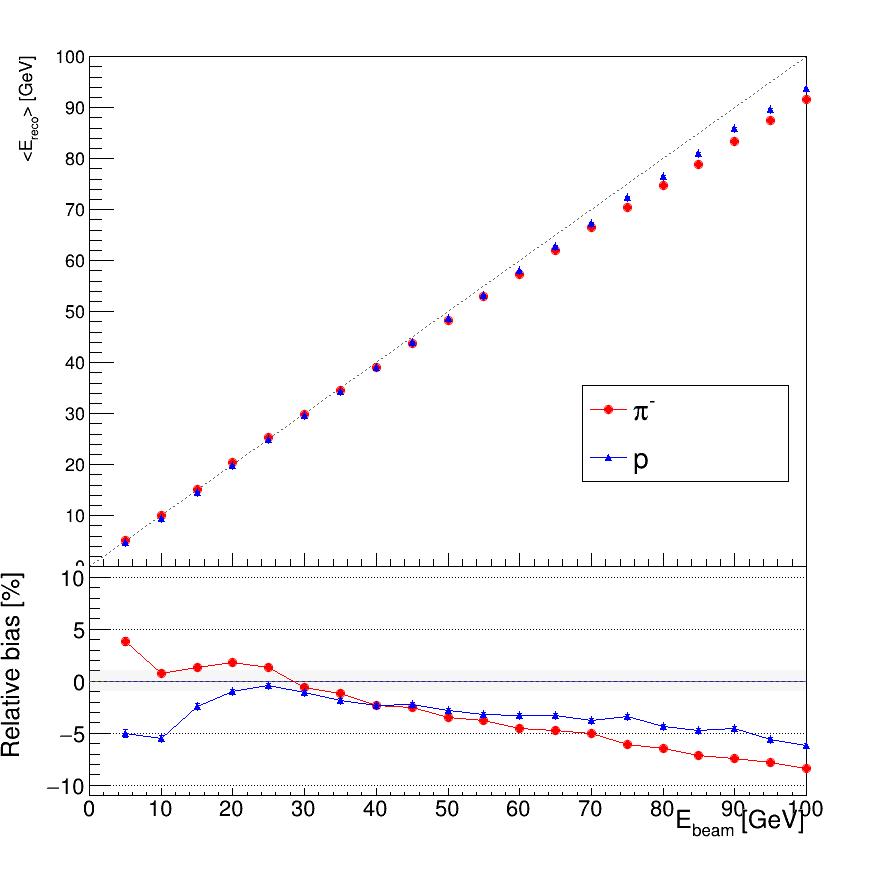
\includegraphics[width=0.78\linewidth]{Fig/PID_Lin_n_Dev_chi2.png}
\caption{Linéarité de la reconstruction et biais relatif pour la chaîne \textbf{PID + méthode paramétrique}.}
\label{fig:linearite_pid_param_new}
\end{figure}

\subsection*{Résolution énergétique}

La Figure~\ref{fig:resolution_pid_param_new} montre la résolution relative \(\sigma(E)/E\).

Le comportement suit la décroissance attendue avec l’énergie, passant d’environ \(19\,\%\) à basse énergie à des valeurs proches de \(9\,\%\) autour de \SI{100}{GeV}. Les performances restent donc globalement bonnes.

Les protons conservent une légère avance sur les pions sur la quasi-totalité du domaine énergétique, avec un écart modéré mais systématique. La hiérarchie observée est similaire à celle du cas BDT.

Cependant, à énergie élevée, la résolution reste légèrement moins bonne que celle obtenue avec la régression LightGBM.

\begin{figure}[!ht]
\centering
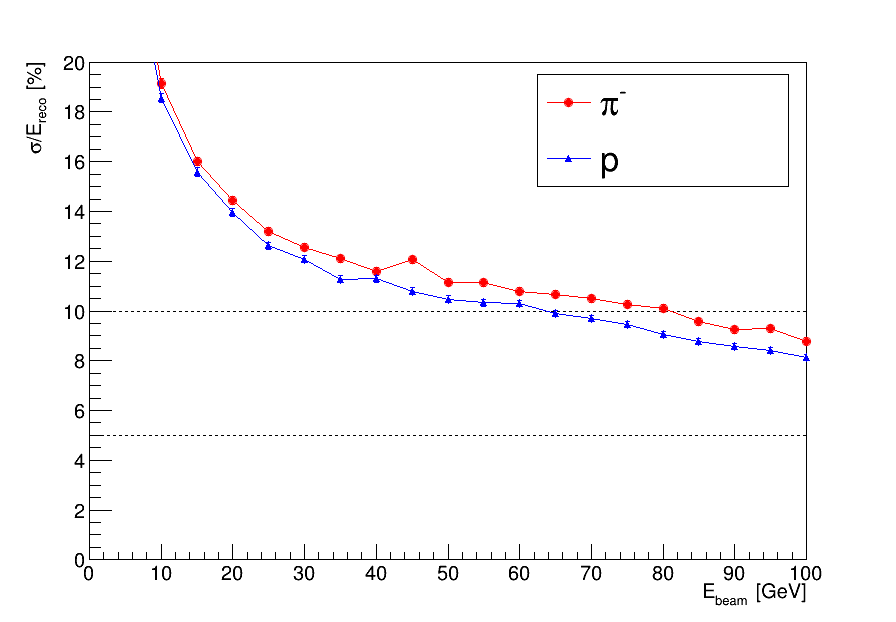
\includegraphics[width=0.78\linewidth]{Fig/PID_Resolution_relative_chi2.png}
\caption{Résolution relative \(\sigma(E)/E\) pour la chaîne \textbf{PID + méthode paramétrique}.}
\label{fig:resolution_pid_param_new}
\end{figure}

\subsection*{Interprétation physique}

Ces résultats montrent que la méthode paramétrique conserve une bonne robustesse statistique, même en présence d’une étape de PID en amont. Les performances restent proches de celles du scénario idéal, ce qui confirme la pertinence physique des observables basées sur les trois seuils semi-digitaux.

La sous-réponse croissante à haute énergie reflète néanmoins les limites intrinsèques de la paramétrisation analytique retenue. Lorsque les gerbes deviennent plus développées et plus fluctuantes, une combinaison polynomiale simple des compteurs \(N_1\), \(N_2\) et \(N_3\) ne suffit plus toujours à corriger les effets de saturation ou de non-linéarité.

La légère supériorité des protons suggère à nouveau une réponse plus régulière de leurs gerbes dans le calorimètre.

\subsection*{Bilan}

La chaîne \textbf{PID + méthode paramétrique} fournit une reconstruction d’énergie compétitive, simple à mettre en œuvre et physiquement interprétable. Elle reste toutefois limitée par un biais croissant aux hautes énergies et par une résolution légèrement inférieure à celle obtenue avec la stratégie PID + BDT. Elle constitue donc une solution robuste, mais moins performante que l’approche fondée sur l’apprentissage supervisé.
%%%%%%%%%%%%%%%%%%%%%%%%%%%%%%%%%%%%%%%%%%%%%%%%%%%%%
\section{Calibration pion appliquée à toutes les espèces}
\label{subsec:param_pion_to_all_new}

La troisième stratégie étudiée sert de référence simplifiée. Elle consiste à utiliser une unique calibration déterminée sur les pions \(\pi^-\), puis à l’appliquer indistinctement à tous les événements du faisceau mixte, y compris lorsqu’ils correspondent à des protons.

Une telle méthode ne nécessite aucune étape préalable d’identification des particules. Elle représente donc une solution opérationnellement simple, mais potentiellement sensible aux différences physiques entre espèces hadroniques.

L’objectif de cette étude est de quantifier le gain réel apporté par le PID en comparant cette calibration unique aux deux approches précédentes.

\subsection*{Linéarité de la réponse}

La Figure~\ref{fig:linearite_pion_all_new} montre la réponse moyenne reconstruite et le biais relatif obtenu avec cette calibration universelle.

Les pions, utilisés pour déterminer les coefficients, restent naturellement les mieux reconstruits. Leur biais reste modéré sur une large partie du domaine énergétique, avec une réponse proche de la diagonale idéale jusqu’aux énergies intermédiaires.

En revanche, les protons présentent un décalage systématique négatif beaucoup plus marqué. Après une région relativement correcte autour de \SIrange{20}{30}{GeV}, la sous-réponse augmente progressivement avec l’énergie pour atteindre environ \(-6\,\%\) à \SI{100}{GeV}.

Cette différence entre espèces met clairement en évidence qu’une calibration optimisée pour les pions ne peut être transposée sans perte aux protons.

\begin{figure}[!ht]
\centering
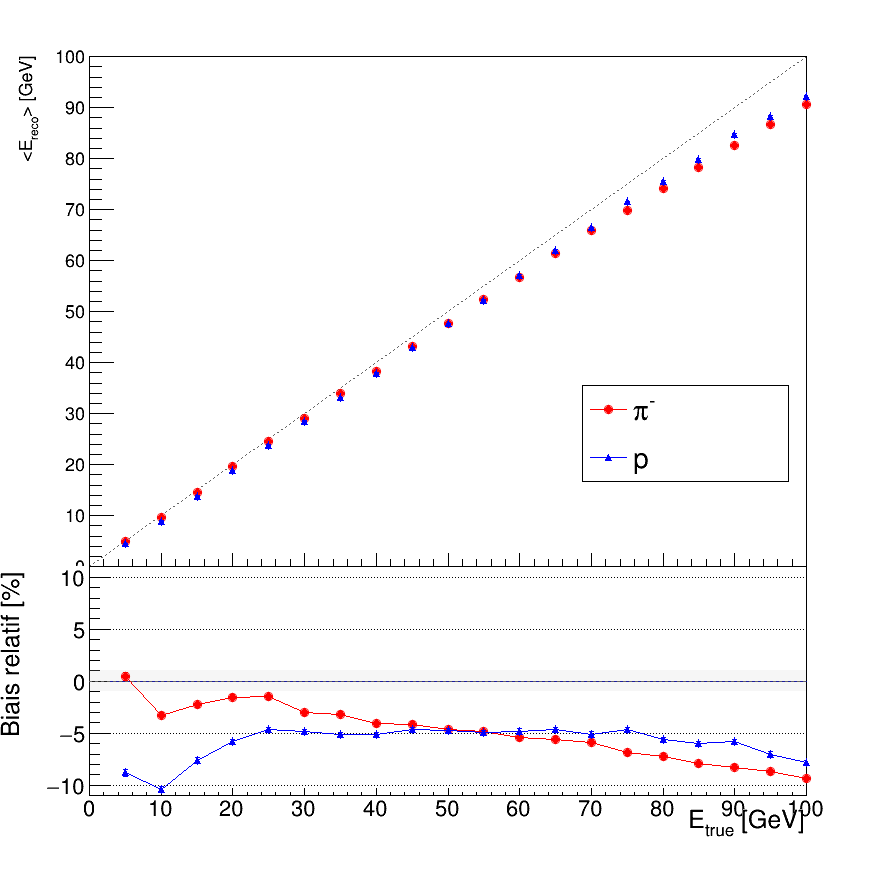
\includegraphics[width=0.78\linewidth]{Fig/PID_Lin_n_Dev_chi2_pion.png}
\caption{Linéarité de la reconstruction et biais relatif lorsqu’une calibration ajustée sur les pions est appliquée à toutes les espèces.}
\label{fig:linearite_pion_all_new}
\end{figure}

\subsection*{Résolution énergétique}

La Figure~\ref{fig:resolution_pion_all_new} présente la résolution relative \(\sigma(E)/E\).

Les performances restent globalement correctes et suivent la décroissance attendue avec l’énergie. À \SI{100}{GeV}, la résolution atteint des valeurs proches de \(8\) à \(9\,\%\), comparables aux autres approches.

Les protons gardent même une légère avance sur les pions en résolution pure, malgré leur biais systématique plus important. Cela montre qu’une bonne résolution ne garantit pas nécessairement une réponse correctement calibrée.

\begin{figure}[!ht]
\centering
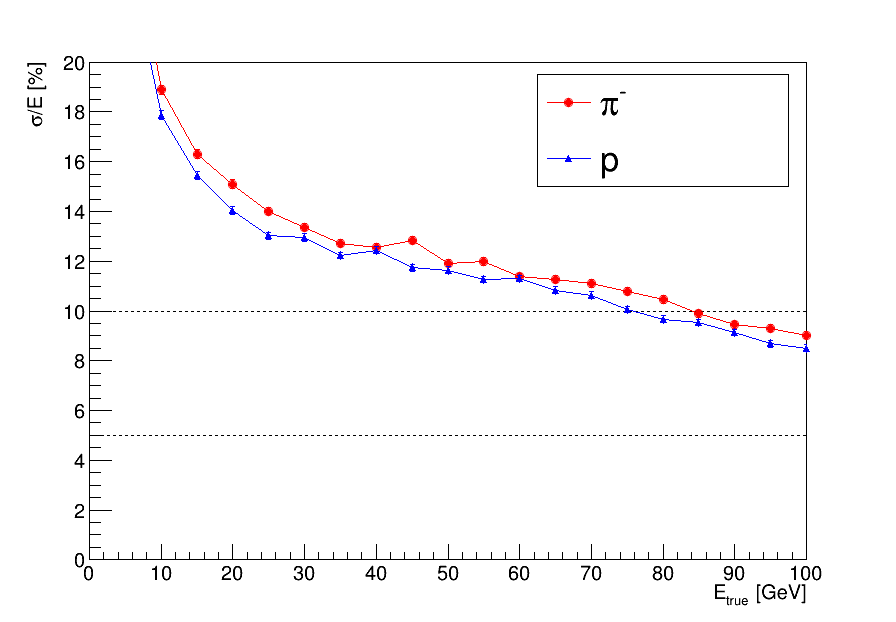
\includegraphics[width=0.78\linewidth]{Fig/PID_Resolution_relative_chi2_pion.png}
\caption{Résolution relative \(\sigma(E)/E\) obtenue avec une calibration pion appliquée à tous les événements.}
\label{fig:resolution_pion_all_new}
\end{figure}

\subsection*{Interprétation physique}

Ce comportement est cohérent avec les différences de développement des gerbes hadroniques selon l’espèce incidente. Les protons ne déposent pas leur énergie selon exactement les mêmes profils que les pions : profondeur moyenne d’interaction, fraction électromagnétique et densité locale peuvent différer.

Une calibration unique absorbe correctement la réponse moyenne des pions, mais ne capture pas ces spécificités pour les protons, d’où le biais observé.

Cette étude démontre ainsi que le PID n’améliore pas seulement l’étiquetage des événements : il permet aussi de sélectionner une calibration énergétique adaptée, ce qui réduit directement les biais systématiques.

\subsection*{Bilan}

L’approche par calibration unique constitue une base simple et raisonnablement performante en résolution, mais elle introduit un biais dépendant de l’espèce, particulièrement visible pour les protons aux hautes énergies.

Elle représente donc une solution de référence utile, mais inférieure aux stratégies exploitant explicitement l’identification des particules avant la reconstruction de l’énergie.
%%%%%%%%%%%%%%%%%%%%%%%%%%%%%%%%%%%%%%%%%%%%%%%%%%%%%%
\section{Comparaison globale des approches}
\label{subsec:comparaison_mixte}

Les trois stratégies étudiées permettent toutes de reconstruire l’énergie incidente avec des performances globalement satisfaisantes. Des différences nettes apparaissent toutefois lorsqu’on compare simultanément la linéarité de la réponse, la résolution énergétique et la robustesse vis-à-vis du mélange d’espèces.

L’intérêt de cette comparaison n’est donc pas uniquement de désigner la méthode la plus performante, mais d’identifier le meilleur compromis entre précision calorimétrique, simplicité de mise en œuvre et capacité d’adaptation à un environnement expérimental réaliste.

\subsection*{Linéarité et biais}

La chaîne \textbf{PID + LightGBM} fournit la réponse la plus proche du comportement idéal. Le biais reste faible sur la majeure partie du domaine énergétique, généralement contenu dans quelques pourcents, avec seulement une légère surestimation aux basses énergies et une faible sous-réponse à \SI{100}{GeV}.

La stratégie \textbf{PID + méthode paramétrique} conserve une bonne linéarité globale, mais présente une dérive négative progressive lorsque l’énergie augmente. Cette tendance traduit les limites d’une paramétrisation analytique fixe face à l’évolution de la morphologie des gerbes avec l’énergie.

Enfin, la \textbf{calibration pion appliquée à toutes les espèces} met en évidence un biais dépendant de la nature de la particule. Les pions restent correctement reconstruits, tandis que les protons subissent une sous-estimation systématique croissante avec l’énergie.

Ainsi, l’identification préalable des particules réduit clairement les biais de calibration inter-espèces et améliore la stabilité globale de la réponse.

\subsection*{Résolution énergétique}

Les trois approches présentent une décroissance régulière de la résolution relative avec l’énergie, conforme au comportement attendu d’un calorimètre hadronique.

La chaîne \textbf{PID + LightGBM} atteint les meilleures performances globales, avec une résolution proche de \(8\,\%\) aux plus hautes énergies.

La méthode \textbf{PID + paramétrique} reste légèrement en retrait, avec des valeurs proches de \(9\,\%\) autour de \SI{100}{GeV}.

La \textbf{calibration pion universelle} conserve une résolution du même ordre de grandeur, ce qui montre que la dispersion statistique reste correctement maîtrisée même lorsqu’un biais moyen subsiste.

Ces observations soulignent qu’une bonne résolution ne garantit pas, à elle seule, une reconstruction correctement calibrée : la maîtrise du biais constitue un critère tout aussi essentiel.

\subsection*{Apport spécifique du PID}

L’un des enseignements majeurs de cette étude est que le PID n’intervient pas uniquement comme outil de classification, mais également comme levier direct d’amélioration de la reconstruction calorimétrique.

En distinguant les pions des protons avant l’estimation de l’énergie, il devient possible d’appliquer une calibration cohérente avec la physique propre à chaque espèce. Le bénéfice se manifeste principalement par une réduction des biais systématiques, particulièrement visible dans la comparaison avec la calibration unique issue des pions.

Les erreurs résiduelles du classificateur limitent naturellement ce gain potentiel, mais leur impact reste modéré dans les performances observées ici.

\subsection*{Choix de la stratégie optimale}

Au regard des résultats obtenus :

\begin{itemize}
    \item la chaîne \textbf{PID + LightGBM} apparaît comme la solution la plus performante et la plus polyvalente dans le cadre de cette étude ;
    
    \item la chaîne \textbf{PID + paramétrique} constitue une alternative robuste, plus simple et plus directement interprétable ;
    
    \item la \textbf{calibration pion unique} peut servir de référence minimale ou de solution de secours, mais reste pénalisée par un biais dépendant de l’espèce incidente.
\end{itemize}

Le choix final dépend donc du contexte visé : recherche de performance maximale, besoin de simplicité opérationnelle, ou exigence de contrôle systématique renforcé.

\subsection*{Bilan}

Dans un environnement expérimental réaliste, la combinaison d’un PID supervisé et d’un estimateur d’énergie spécialisé apparaît comme la stratégie la plus pertinente. Elle permet d’exploiter simultanément la richesse topologique du SDHCAL pour identifier la particule incidente et améliorer la précision de la mesure énergétique.

Ces résultats confirment plus largement que, dans un calorimètre hautement granulaire, identification des particules et reconstruction d’énergie gagnent à être pensées conjointement plutôt que comme deux problèmes indépendants.
%%%%%%%%%%%%%%%%%%%%%%%%%%%%%%%%%%%%%%%%%%%%%%%%%%%%%
\section{Synthèse et conclusion}
\label{subsec:conclusion_mixte}

Ce chapitre avait pour objectif d’évaluer la reconstruction de l’énergie dans une configuration plus réaliste que les études précédentes, où l’espèce de la particule incidente n’est plus supposée connue a priori. Les événements considérés proviennent d’un faisceau mixte composé de pions \(\pi^-\) et de protons \(p\), de sorte que l’estimation de l’énergie repose sur une chaîne complète intégrant une étape préalable d’identification des particules.

Trois stratégies complémentaires ont été comparées :

\begin{itemize}
    \item un schéma \textbf{PID + régression LightGBM}, dans lequel le classificateur sélectionne un estimateur supervisé spécialisé ;
    
    \item un schéma \textbf{PID + méthode paramétrique}, fondé sur une calibration analytique dépendant de l’espèce reconstruite ;
    
    \item une \textbf{calibration unique ajustée sur les pions}, appliquée indistinctement à tous les événements.
\end{itemize}

Les résultats montrent que la chaîne \textbf{PID + LightGBM} fournit les meilleures performances globales dans le cadre de cette étude. Elle combine une excellente linéarité, des biais faibles sur l’ensemble du domaine énergétique, ainsi qu’une résolution atteignant environ \(8\,\%\) aux plus hautes énergies. Cette stratégie apparaît ainsi comme la plus efficace pour exploiter conjointement les informations de classification et de reconstruction disponibles dans le SDHCAL.

La méthode \textbf{PID + paramétrique} demeure compétitive et conserve l’avantage d’une interprétation physique directe. Ses performances restent solides sur l’ensemble du domaine étudié, bien qu’une sous-réponse croissante apparaisse aux hautes énergies, traduisant les limites d’une paramétrisation analytique fixe face à des gerbes plus développées et plus fluctuantes.

La \textbf{calibration pion universelle}, enfin, montre qu’une reconstruction globalement correcte peut être obtenue sans PID explicite, mais au prix d’un biais systématique pour les protons. Ce résultat met clairement en évidence l’intérêt d’une identification préalable des particules afin de sélectionner une calibration adaptée à la physique de l’espèce incidente.

Au-delà de la comparaison algorithmique, cette étude souligne un point essentiel : dans un calorimètre hadronique hautement granulaire, l’identification des particules et la reconstruction d’énergie ne doivent pas être considérées comme deux problèmes indépendants. Elles constituent au contraire deux étapes étroitement couplées d’une même chaîne d’analyse.

Le PID améliore directement la qualité de la mesure calorimétrique en réduisant les biais inter-espèces, tandis qu’une reconstruction d’énergie plus précise peut, en retour, renforcer certaines stratégies globales de reconstruction d’événements, notamment dans les approches de type \emph{Particle Flow}.

En conclusion, les résultats obtenus confirment que le SDHCAL possède un fort potentiel non seulement pour l’identification hadronique, mais également pour une reconstruction énergétique performante en environnement mixte. Ils ouvrent la voie à des développements futurs combinant simultanément PID, estimation d’énergie et exploitation directe des hits bruts au moyen de méthodes d’apprentissage plus avancées.